\subsection{JAM with a NFW Dark Matter Halo}

\subsubsection{Sampling with a Markov Monte Carlo Chain}

[TO DO]

\begin{figure*}
\centering
\includegraphics[width=0.9\linewidth]{fig/B4_contour_plot_short.ps}
\caption{??? Preliminary crappy caption: Result of the MCMC sampling of the parameter space for a model with NFW halo and constant velocity anisotropy. Green and blue shows the priors. Grey diamonds are the models shown in next figure. ??? [TO DO: nice caption]}
\label{fig:???}
\end{figure*}

\begin{figure*}
\centering
\begin{subfigure}{\textwidth}
  \centering
  \includegraphics[width=0.8\linewidth]{fig/B4_rms_error_curves.ps}
  \caption{???}
  \label{fig:???}
\end{subfigure}
\begin{subfigure}{.5\textwidth}
  \centering
  \includegraphics[width=0.9\linewidth]{fig/B4_jam_profiles_errors_short_vcirc.ps}
  \caption{????????}
  \label{fig:???}
\end{subfigure}%
\begin{subfigure}{.5\textwidth}
  \centering
  \includegraphics[width=0.9\linewidth]{fig/B4_jam_profiles_errors_short_projmass.ps}
  \caption{???}
  \label{fig:???}
\end{subfigure}
\caption{??? Preliminary crappy caption: 12 samples from the parameter pdf found with the MCMC above for the model with NFW halo and constant velocity anisotropy. Big red dot shows the Einstein mass with a 10\% error (used in fit). ??? [TO DO: nice caption]}
\label{fig:???}
\end{figure*}



\subsubsection{Predicting the Rotation Curve at larger Radii}

[TO DO]

\begin{figure*}
\centering
\includegraphics[width=0.7\linewidth]{fig/B4_rms_rot_curves_best_model.ps}
\caption{??? Preliminary crappy caption: Model: NFW halo and constant velocity anisotropy, using the the mean / peak values of the MCMC result in the above pdf for the model parameters. Fitting one more free parameter to the rotation curve in the inner regions, predicting the rotation curve and dispersion at larger radii. Green dots are gas kinematics. ??? [TO DO: nice caption]}
\label{fig:???}
\end{figure*}
